\documentclass{article}

\usepackage[utf8]{inputenc}
\usepackage{amsmath}
\usepackage{amsfonts}
\usepackage{amssymb}
\usepackage{graphicx}
\usepackage[table,xcdraw]{xcolor}
\usepackage[bookmarks,hypertexnames=false,debug,linktocpage=true,hidelinks]{hyperref}
\usepackage{placeins}
\usepackage{tabularx}

\hypersetup{
    colorlinks,
    linktoc=all,
    linkcolor={blue},
    citecolor={blue},
    urlcolor={blue}
}

\usepackage{tikz}
\newcommand*\circled[1]{\tikz[baseline=(char.base)]{
            \node[shape=circle,draw,inner sep=2pt] (char) {#1};}}


\graphicspath{ {./media/} }

\renewcommand{\contentsname}{Indice}

\makeatletter
\newcommand*{\rom}[1]{\expandafter\@slowromancap\romannumeral#1@}
\makeatother

\usepackage[a4paper,top=2cm,bottom=2cm,left=2cm,right=2cm]{geometry}

\setcounter{section}{-1}

\title{\textbf{\Huge Specifica dei Requisiti}}
\author{Matteo Girardi, Vasile Donmovil, Antonio Scendrate Gattico \\ Gruppo T45 - Deliverable D2}
\date{2022}

\begin{document}

\maketitle

\clearpage
\tableofcontents
\clearpage

% #### Scopo del documento ####
\section{Scopo del documento}
\begin{description}
	\item[] Il presente documento illustra la specifica dei requisiti di sistema del progetto, utilizzando anche rappresentazioni grafiche, come diagrammi UML e tabelle strutturate; i requisiti verranno descritti usando sia linguaggio naturale sia in linguaggi più formali e strutturati.
	\item[] Grazie a diagrammi di contesto e dei componenti verrà presentato il design del sistema.
\end{description}
\clearpage

% #### Req. funz ####
\section{Requisiti Funzionali}
\begin{description}
	\item[] Si individuano 4 attori che interagiranno con la webapp:
	\begin{itemize}
		\item  Utente Non Registrato
		\item  Utente Registrato
		\item  Utente Amministratore
		\item  Servizio di Notifica
	\end{itemize}
\end{description}


% # Utente non registrato #
\subsection{Utente Non Registrato}
\renewcommand\thesubsubsection{RF \arabic{subsubsection}}

\subsubsection{Visualizzazione Date}\label{rf_1}
\begin{description}
	    
	\begin{figure}[htp]
		\centering
		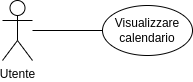
\includegraphics[]{rf1.png}
	\end{figure}
	     
	\item L'utente può visualizzare un calendario con evidenziati i giorni in cui sono disponibili gli appuntamenti. 
\end{description}


% # Utente registrato #
\subsection{Utente Registrato}

\subsubsection{Visualizzazione Date}\label{rf_1}
\begin{description}
	    
	\begin{figure}[htp]
		\centering
		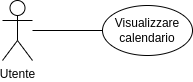
\includegraphics[]{rf1.png}
	\end{figure}
	    
	\item L'utente può visualizzare un calendario con evidenziati i giorni in cui sono disponibili gli appuntamenti. 
\end{description}

\subsubsection{Prenotazione Sala}\label{rf_2}
\begin{description}
	
	\begin{figure}[htp]
		\centering
		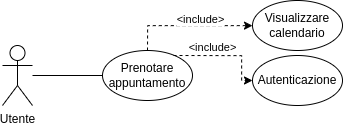
\includegraphics[]{rf2.png}
	\end{figure}
		
	\item Un utente è in grado di prenotare un appuntamento, consultando il calendario dove sono evidenziate le date disponibili. L'utente può concludere con successo una prenotazione solamente dopo aver effettuato il Login al sistema.   	
\end{description}

\clearpage

\subsubsection{Gestione prenotazioni}\label{rf_3}
\begin{description}
	
	\begin{figure}[htp]
		\centering
		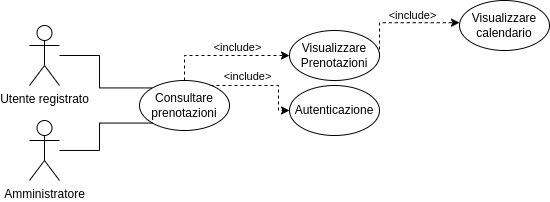
\includegraphics[width=\textwidth]{rf3.png}
	\end{figure}
	
	\item L'utente può consultare le proprie prenotazioni, precedentemente prenotate, così da poter capire quando e dove avverranno.
\end{description}

\subsubsection{Annullare una Prenotazione}\label{rf_4}
\begin{description}
	
	\begin{figure}[htp]
		\centering
		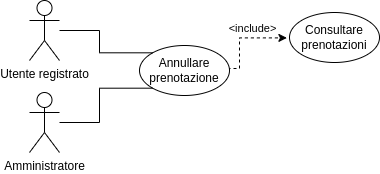
\includegraphics[]{rf4.png}
	\end{figure}
	
	\item L'utente può annullare le proprie prenotazioni precedentemente effettuate.
\end{description}


\subsubsection{Login}\label{rf_5}
\begin{description}
	
	\begin{figure}[htp]
		\centering
		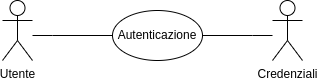
\includegraphics[]{rf5.png}
	\end{figure}
	
	\item L'utente che possiede credenziali idonee può utilizzarle per autenticarsi alla piattaforma, così da poter interagire con essa da utente registrato.
\end{description}

\clearpage

\subsubsection{Logout}\label{rf_6}
\begin{description}
	
	\begin{figure}[htp]
		\centering
		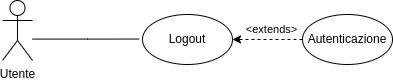
\includegraphics[]{rf6.png}
	\end{figure}
	
	\item Una volta che l'utente ha eseguito l'accesso alla piattaforma è anche in grado di terminare la sessione, di fatto tornando un utente non registrato agli occhi di quest'ultima. L'utente deve aver effettuato il login precedentemente. 
\end{description}


\renewcommand\thesubsubsection{RF 8}
\subsubsection{Gestione Account}\label{rf_8}
\begin{description}
	
	\begin{figure}[htp]
		\centering
		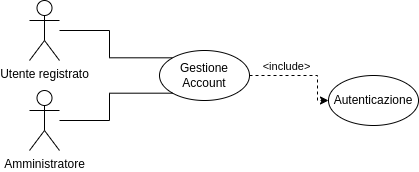
\includegraphics[]{rf8.png}
	\end{figure}	
		
	\item L'utente che ha effettuato il login al sistema è anche in grado di consultare i propri dati interni al sistema, potendo anche aggiornare tali dati.
\end{description}

\renewcommand\thesubsubsection{RF 9}
\subsubsection{Rimozione Account}\label{rf_9}
\begin{description}
	
	\begin{figure}[htp]
		\centering
		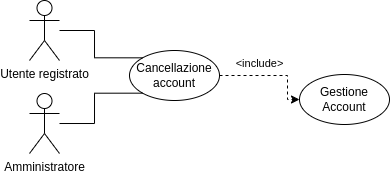
\includegraphics[]{rf9.png}
	\end{figure}
	
	\item L'utente che ha effettuato il login al sistema è anche in grado di cancellare il proprio account, così da terminare la sua capacità di usufruire della piattaforma.
\end{description}

\clearpage

% # ADMIN #
\subsection{Utente Amministratore}

\renewcommand\thesubsubsection{RF \arabic{subsubsection}}
\subsubsection{Visualizzazione Date}\label{rf_1}
\begin{description}
	    
	\begin{figure}[htp]
		\centering
		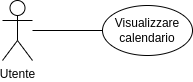
\includegraphics[]{rf1.png}
	\end{figure}
	    
	\item L'utente può visualizzare un calendario con evidenziati i giorni in cui sono disponibili gli appuntamenti. 
\end{description}

\renewcommand\thesubsubsection{RF 3}
\subsubsection{Gestione prenotazioni}\label{rf_3}
\begin{description}
	
	\begin{figure}[htp]
		\centering
		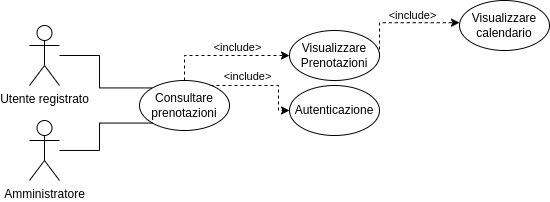
\includegraphics[width=\textwidth]{rf3.png}
	\end{figure}
	
	\item L'utente Amministratore può consultare le prenotazioni effettuate dagli utenti registrati alla piattaforma.
\end{description}

\renewcommand\thesubsubsection{RF 4}
\subsubsection{Annullare una Prenotazione}\label{rf_4}
\begin{description}
	
	\begin{figure}[htp]
		\centering
		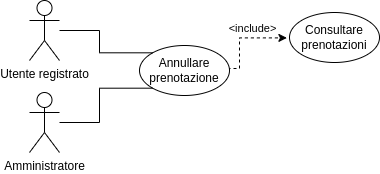
\includegraphics[]{rf4.png}
	\end{figure}
	
	\item L'utente Amministratore può annullare le prenotazioni precedentemente effettuate da parte di altri utenti registrati.
\end{description}

\clearpage

\renewcommand\thesubsubsection{RF 5}
\subsubsection{Login}\label{rf_5}
\begin{description}
	
	\begin{figure}[htp]
		\centering
		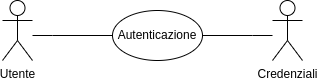
\includegraphics[]{rf5.png}
	\end{figure}
	
	\item L'utente Amministratore che possiede credenziali idonee può utilizzarle per autenticarsi alla piattaforma, così da poter interagire con essa da utente registrato.
\end{description}

\renewcommand\thesubsubsection{RF 6}
\subsubsection{Logout}\label{rf_6}
\begin{description}
	
	\begin{figure}[htp]
		\centering
		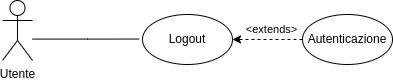
\includegraphics[]{rf6.png}
	\end{figure}
	
	\item Una volta che l'utente Amministratore ha eseguito l'accesso alla piattaforma è anche in grado di terminare la sessione, di fatto tornando un utente non registrato agli occhi di quest'ultima. L'utente deve aver effettuato il login precedentemente. 
\end{description}

\renewcommand\thesubsubsection{RF 7}
\subsubsection{Creazione Nuovo Account}\label{rf_7}
\begin{description}
	
	\begin{figure}[htp]
		\centering
		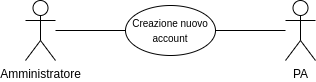
\includegraphics[]{rf7.png}
	\end{figure}
	
	\item L'utente amministratore può creare manualmente un nuovo account utente, somministrando alla Pubblica Amministrazione i dati anagrafici forniti dal donatore (ossia un futuro utilizzatore della piattaforma). Ogni donatore è registrato presso un ente dedicato interno alla PA. Una volta che l'ente accetta la registrazione del donatore al sistema può interagire con esso, effettuando il login.
\end{description}

\clearpage

\renewcommand\thesubsubsection{RF 8}
\subsubsection{Gestione Account}\label{rf_8}
\begin{description}
	
	\begin{figure}[htp]
		\centering
		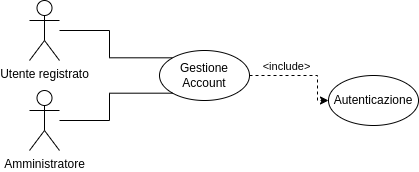
\includegraphics[]{rf8.png}
	\end{figure}	
		
	\item L'utente che ha effettuato il login al sistema è anche in grado di consultare i propri dati interni al sistema, potendo anche aggiornare tali dati. L'utente Amministratore è in grado di consultare informazioni appartenenti agli utenti registrati.
\end{description}

\renewcommand\thesubsubsection{RF 9}
\subsubsection{Rimozione Account}\label{rf_9}
\begin{description}
	
	\begin{figure}[htp]
		\centering
		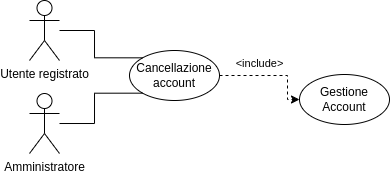
\includegraphics[]{rf9.png}
	\end{figure}
	
	\item L'utente che ha effettuato il login al sistema è anche in grado di cancellare il proprio account, così da terminare la sua capacità di usufruire della piattaforma. L'utente Amministratore è in grado di cancellare l'account di un utente regsitrato.
\end{description}

\renewcommand\thesubsubsection{RF 10}
\subsubsection{Modifica Stato Sala}\label{rf_10}
\begin{description}
	
	\begin{figure}[htp]
		\centering
		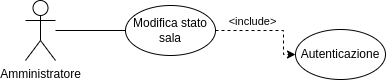
\includegraphics[]{rf10.png}
	\end{figure}
	
	\item L’utente amministratore può modificare lo stato di una specifica sala.
\end{description}

\clearpage

\subsection{Servizio di Notifica SMS/Email}
% ### notifica ###
\renewcommand\thesubsubsection{RF 11}
\subsubsection{Notifica Prenotazione}\label{rf_11}
\begin{description}
	
	\begin{figure}[htp]
		\centering
		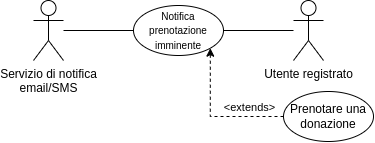
\includegraphics[]{rf11.png}
	\end{figure}
		
	\item Quando la prenotazione è imminente, il servizio di notifica tramite SMS/Email invia un messaggio all'utente riguardo l'evento.
\end{description}
\clearpage


% #### Req. non. funz ####
\section{Requisiti Non Funzionali}
\begin{description}
	\item[] Nel presente capitolo vengono riportati i requisiti non funzionali (RNF) del sistema utilizzando tabelle strutturate e specificando misure facilmente verificabili. 
\end{description}

\renewcommand\thesubsubsection{RNF \arabic{subsubsection}}

\subsubsection{Privacy}\label{rnf_1}
\begin{description}
	\item[]
	    
	% Please add the following required packages to your document preamble:
	% \usepackage{graphicx}
	
	
	\begin{table}[!htbp]
		\begin{tabular} {|>{\raggedright\arraybackslash}m{0.20\linewidth} | >{\raggedright\arraybackslash}m{0.50\linewidth}|>{\raggedright\arraybackslash}m{0.20\linewidth}|}
			\hline
			\textbf{Proprietà}                & \textbf{Descrizione}                                                                                               & \textbf{Misura} \\ \hline
			Minimizzazione dei dati            & I dati devono essere adeguati pertinenti e limitati a quanto necessario rispetto alle finalità del trattamento    & Conforme        \\ \hline
			Esattezza e aggiornamento dei dati & Compresa anche la tempestiva cancellazione dei dati che risultino inesatti rispetto alle finalità del trattamento & Conforme        \\ \hline
			Limitazione della conservazione &
			È necessario provvedere alla conservazione dei dati per un tempo non superiore a quello necessario rispetto agli scopi per i quali è stato effettuato il trattamento &
			Conforme \\ \hline
			Integrità e riservatezza          & Occorre garantire la sicurezza adeguata dei dati personali oggetto di trattamento                                  & Conforme        \\ \hline
		\end{tabular}
	\end{table}
	
	    
\end{description}

\subsubsection{Sicurezza}\label{rnf_2}
\begin{description}
	\item[]
	    
	\begin{table}[!htbp]
		\begin{tabular} {|>{\raggedright\arraybackslash}m{0.20\linewidth} | >{\raggedright\arraybackslash}m{0.50\linewidth}|>{\raggedright\arraybackslash}m{0.20\linewidth}|}
			\hline
			\textbf{Proprietà} & \textbf{Descrizione}                                             & \textbf{Misura}  \\ \hline
			Riservatezza dei dati &
			Per garantire la sicurezza di chi utilizza il servizio, ogni utente avrà solamento accesso ai suoi dati personali &
			Un utente non potrà accedere a dati altrui \\ \hline
			Flusso dati sicuro  & Il flusso di dati opererà sotto protocolli di elevata sicurezza & Traffico cifrato \\ \hline
			Protezione da attacchi &
			Ci si affiderà a servizi terzi per la protezione del servizio da attacchi mirati e tentativi di hacking malevoli &
			Servizio di protezione \\ \hline
		\end{tabular}
	\end{table}
	    
\end{description}

\subsubsection{Scalabilità}\label{rnf_3}
\begin{description}
	\item[]
	    
	\begin{table}[!htbp]
		\begin{tabular} {|>{\raggedright\arraybackslash}m{0.20\linewidth} | >{\raggedright\arraybackslash}m{0.50\linewidth}|>{\raggedright\arraybackslash}m{0.20\linewidth}|}
			\hline
			\textbf{Proprietà} & \textbf{Descrizione}                                                                               & \textbf{Misura}          \\ \hline
			Scalabilità        & La piattaforma viene progettata in modo tale da poter gestire un numero sempre crescente di utenti & Uso di tecnologie ad-hoc \\ \hline
		\end{tabular}
	\end{table}
	    
\end{description}

\subsubsection{Affidabilità}\label{rnf_4}
\begin{description}
	\item[]
	    
	\begin{table}[!htbp]
		\begin{tabular} {|>{\raggedright\arraybackslash}m{0.20\linewidth} | >{\raggedright\arraybackslash}m{0.50\linewidth}|>{\raggedright\arraybackslash}m{0.20\linewidth}|}
			\hline
			\textbf{Proprietà}                                                                                                                           &   
			\textbf{Descrizione}                                                                                                                          &   
			\textbf{Misura} \\ \hline
			Trasmissione affidabile                                                                                                                       &   
			Il sistema di trasmissione dovrà garantire la più alta affidabilità possibile, così da ridurre al minimo la mancata trasmissione dei dati &   
			Logiche di re-invio \\ \hline
		\end{tabular}
	\end{table}
\end{description}

\subsubsection{Resilienza}\label{rnf_5}
\begin{description}
	\item[]
	    
	\begin{table}[!htbp]
		\begin{tabular} {|>{\raggedright\arraybackslash}m{0.20\linewidth} | >{\raggedright\arraybackslash}m{0.50\linewidth}|>{\raggedright\arraybackslash}m{0.20\linewidth}|}
			\hline
			\textbf{Proprietà}    & \textbf{Descrizione}                                                                                 & \textbf{Misura}       \\ \hline
			Operatività garantita & Viene garantita l’operatività anche durante episodi di parziale disservizio di componenti interne & Sistemi di ridondanza \\ \hline
		\end{tabular}
	\end{table}
	    
\end{description}

\clearpage

\subsubsection{Accessibilità}\label{rnf_6}
\begin{description}
	\item[]
	    
	\begin{table}[!htbp]
		\begin{tabular} {|>{\raggedright\arraybackslash}m{0.20\linewidth} | >{\raggedright\arraybackslash}m{0.50\linewidth}|>{\raggedright\arraybackslash}m{0.20\linewidth}|}
			\hline
			\textbf{Proprietà}                                                                                                        &   
			\textbf{Descrizione}                                                                                                       &   
			\textbf{Misura} \\ \hline
			Facile fruizione del servizio                                                                                              &   
			Permettere al servizio di venire usufruito dalla più grande varietà di dispositivi possibile                             &   
			Servizio fornito come sito web \\ \hline
			Compatibilità del servizio                                                                                                &   
			Grande compatibilità coi dispositivi senza compromettere nè l’esperienza di navigazione nè la sicurezza dell’utente &   
			Tecnologie ad-hoc \\ \hline
		\end{tabular}
	\end{table}
	    
\end{description}

\subsubsection{Monitoraggio}\label{rnf_7}
\begin{description}
	\item[]
	    
	\begin{table}[!htbp]
		\begin{tabular} {|>{\raggedright\arraybackslash}m{0.20\linewidth} | >{\raggedright\arraybackslash}m{0.50\linewidth}|>{\raggedright\arraybackslash}m{0.20\linewidth}|}
			\hline
			\textbf{Proprietà}                                                        &   
			\textbf{Descrizione}                                                       &   
			\textbf{Misura} \\ \hline
			Logging \& Monitoring                                                      &   
			Si registrano e analizzano gli accessi al servizio e gli eventi pertinenti &   
			Meccanismo nativo per la registrazione e il monitoraggio su file di testo \\ \hline
		\end{tabular}
	\end{table}
	    
\end{description}

\subsubsection{Multilingua}\label{rnf_8}
\begin{description}
	\item[]
	    
	\begin{table}[!htbp]
		\begin{tabular} {|>{\raggedright\arraybackslash}m{0.20\linewidth} | >{\raggedright\arraybackslash}m{0.50\linewidth}|>{\raggedright\arraybackslash}m{0.20\linewidth}|}
			\hline
			\textbf{Proprietà} & \textbf{Descrizione}                                                 & \textbf{Misura}                                  \\ \hline
			Multilingua         & Lingue previste su tutte le schermate di cui è composto il software & Schermate dispobili in lingua inglese e italiana \\ \hline
		\end{tabular}
	\end{table}
	    
\end{description}

\clearpage

% #### Anal. Contesto ####
\section{Analisi del Contesto}
\begin{description}
	\item[] Nel presente capitolo viene discusso il contesto di funzionamento del sistema, fornendo una descrizione testuale e una rappresentazione grafica basata su Context Diagram.
	
	Nella seguente parte della sezione vengono presentati gli attori e i sistemi esterni con cui BloodStream si interfaccerà. 
\end{description}

\subsection{Utenti e Sistemi esterni}
\begin{itemize}

\item \textbf{Utente}: colui che fa uso del portale per prenotare appuntamenti per donare il sangue. Il RF5 (Login) identifca l'utente non registrato e l'utente registrato.

\item \textbf{Amministratore}: colui che detiene privilegi più elevati, in grado di influire sull'esperienza d'uso degli altri utenti.

\item \textbf{Servizio di Notifica}: l'ente a cui ci si rivolte per assolvere il compito di notificare l'utente riguardo una prenotazione imminente.

\item \textbf{PA} (Pubblica Amministrazione): l'ente a cui ci si rivolge per registrare nuovi utenti all'elenco dei donatori. 
\end{itemize}

\subsection{Diagramma di contesto}
\begin{description}


\begin{figure}[htp]
		\centering
		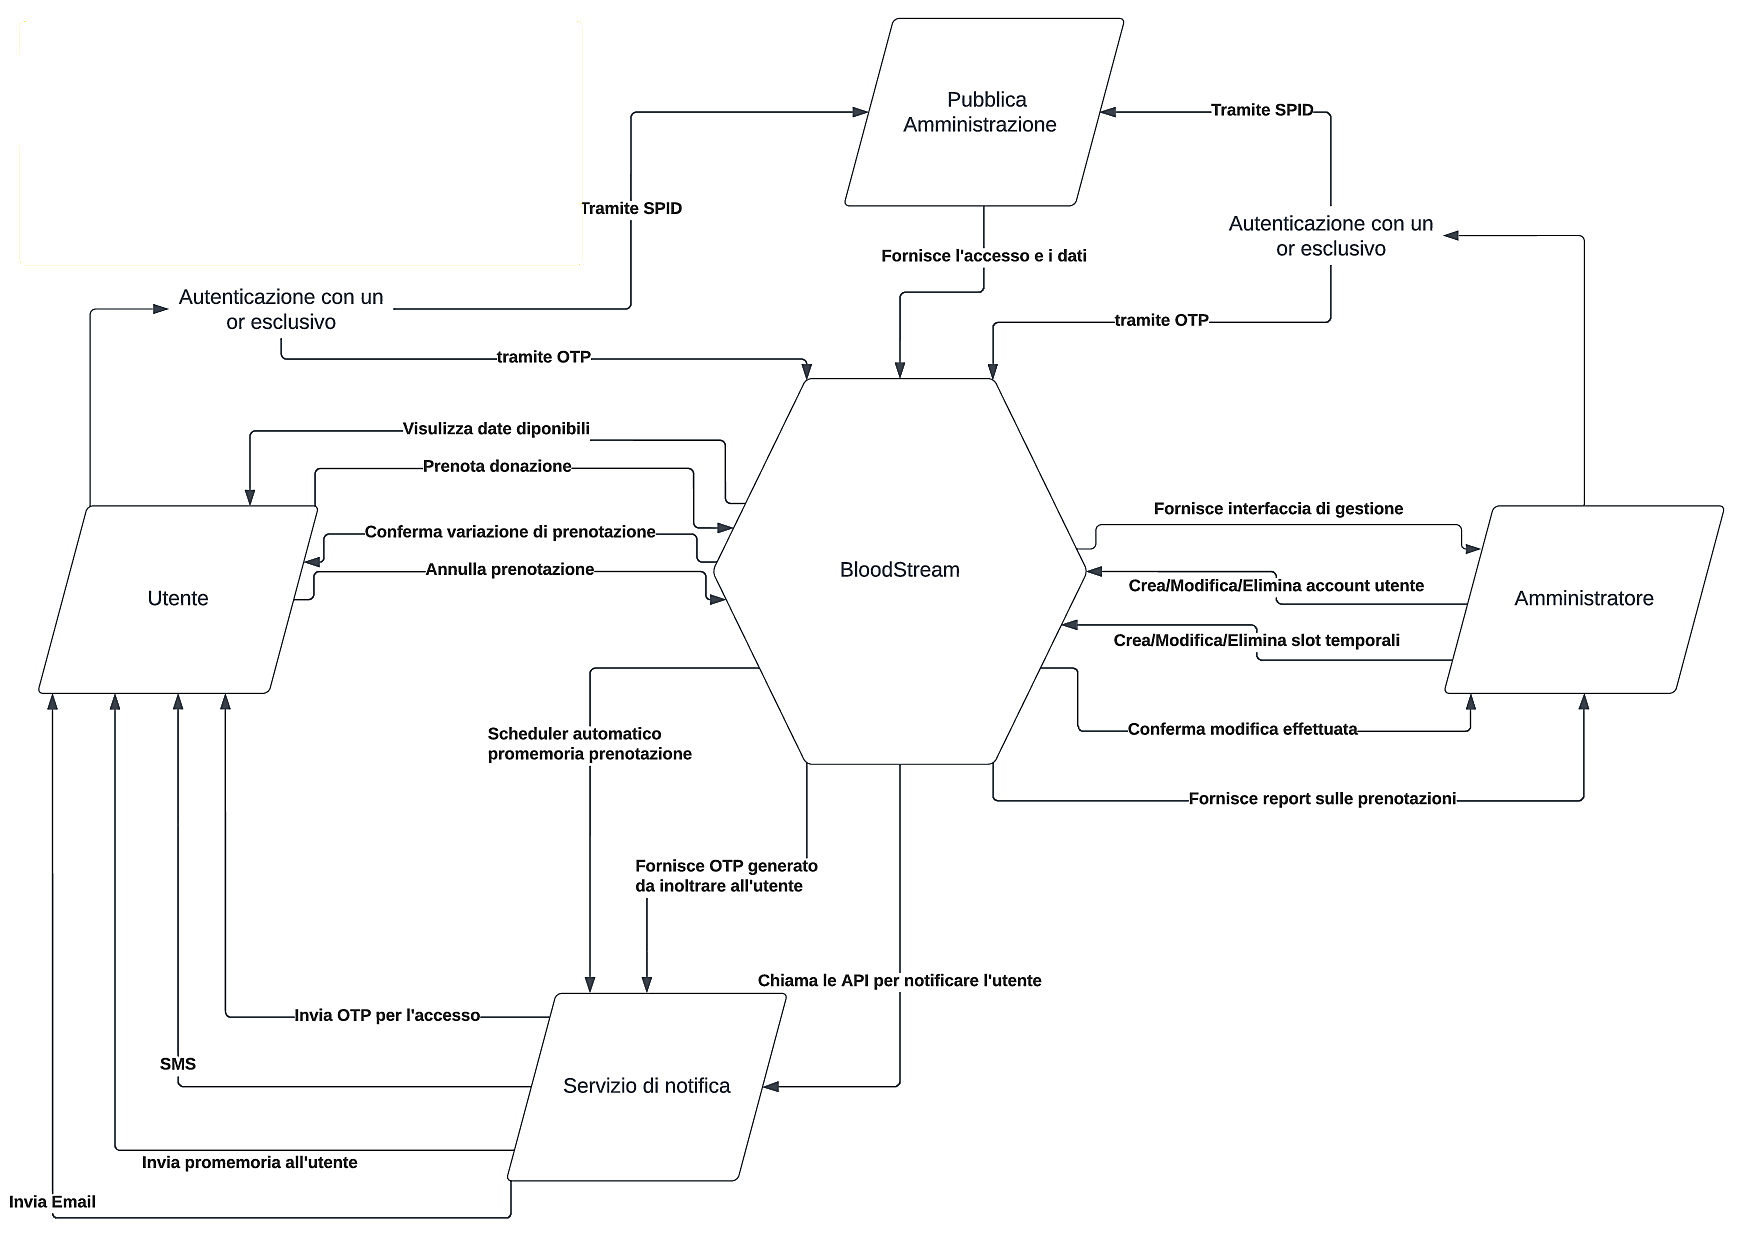
\includegraphics[width=\textwidth]{context-diag.png}
	\end{figure}

\item[] Sia l’utente che l’amministratore eseguono l’autenticazione sul sito tramite OTP oppure passando tramite la pubblica amministazione (SPID) secondo il RF5 e il RF6, l’utente (anche senza autenticazione) ha accesso alla visualizzazione degli slot disponibili (RF1), ma solo una volta autenticato ha accesso alla possibilità di prenotare la sala donazioni RF2 da cui può anche disdire le prenotazioni già effettuate (RF4). \\ Gli amministratori possono modificiare le prenotazioni di qualisiasi utente registrato (mentre l’utente può modificare solo le proprie).
\end{description}


\clearpage

% #### Anal. Compoonent. ####
\section{Analisi dei Componenti}
\subsection{Definizione dei componenti}

\subsection{Diagramma dei componenti}

\begin{figure}[htp]
		\centering
		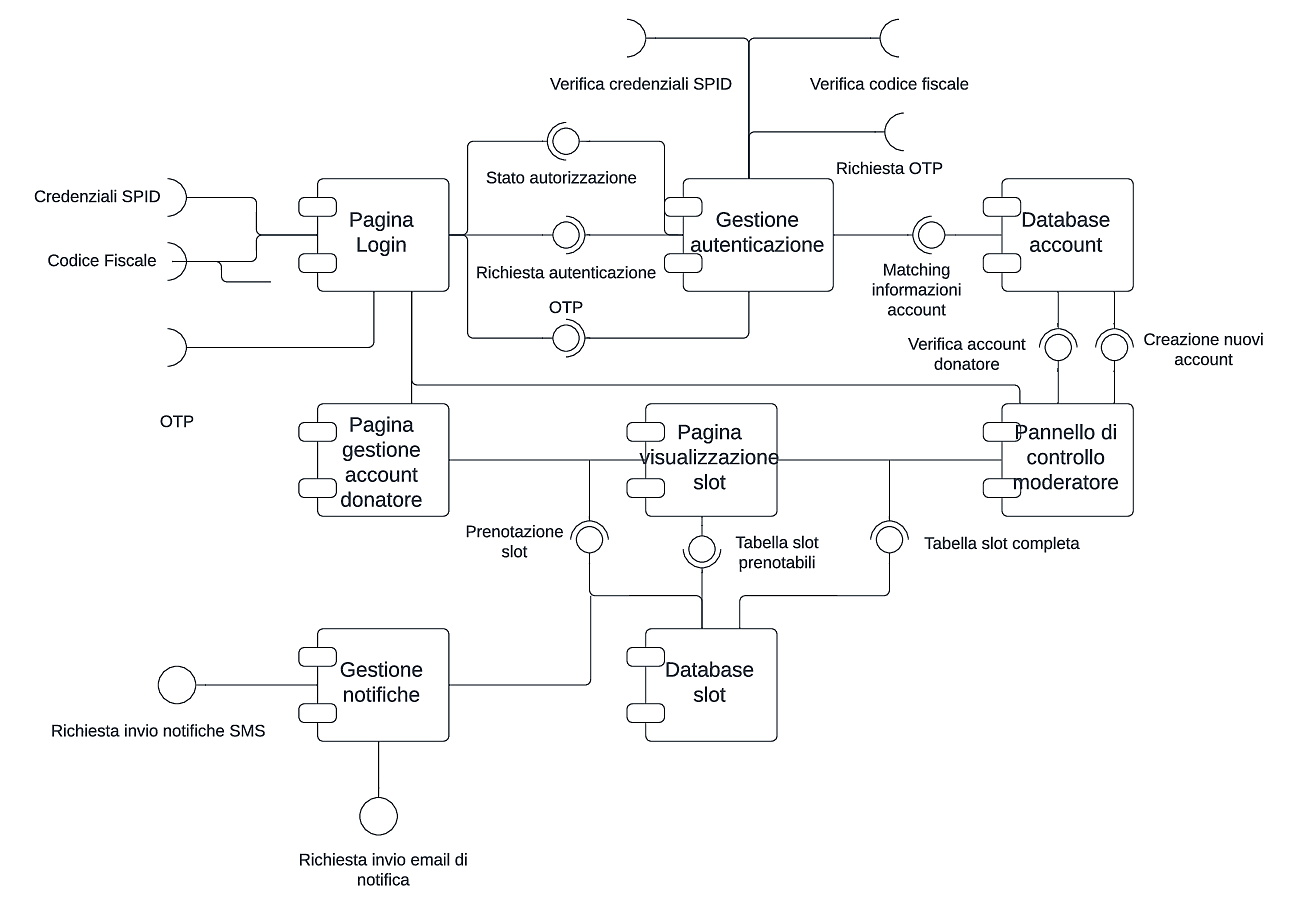
\includegraphics[width=\textwidth]{interface.png}
	\end{figure}

\end{document}